\chapter{Introduction}\label{c1}
\section{Notation and definitions}\label{c1s1}
We will follow the contemporary mathematical style of using unadorned symbols for vectors and
matrices. The nature of a symbol will be determined by its definition and not appearance. For
example, $x$ could be a real number or a point in $\sor^n$ depending on the context. Random
variables will be denoted by capital letters and their realizations by small letters.

A matrix with entries $a_{ij}$ will sometimes be denoted by $((a_{ij}))$.

If $f$ is a function of $n$ variables, $x_1, \ldots, x_n$ then its gradient is defined as
\begin{equation}\label{c1s1e1}
Df := \left(\frac{\partial f}{\partial x_1}, \ldots, \frac{\partial f}{\partial x_n}\right).
\end{equation}
The hessian of $f$ is
\begin{equation}\label{c1s1e2}
(D^2 f)_{ij} := \frac{\partial^2 f}{\partial x_i \partial x_j}.
\end{equation}

\section{Bayesian curve fitting}\label{c1s2}
The problem consists of using the data $\{(x_i, t_i) : 1 \le i \le n\}$ to find the value
of $t$ when a new $x$ is given. We shall fit the data using the polynomial
\begin{equation}\label{c1s2e1}
y(x, w) = \sum_{i=0}^M w_i x^i.
\end{equation}
The polynomial coefficients $w_0, \ldots, w_M$ can be considered to be components of a 
vector $w \in \sor^M$. We assume that for a given value of $x_i$, the target $t_i$ has a 
gaussian distribution with mean $y(x, w)$ and precision $\beta$ (or variance $\beta^{-1}$).
Thus,
\begin{equation}\label{c1s2e2}
p(t_i | x_i, w, \beta) = \mathcal{N}(t | y(x_i, w), \beta^{-1/2}).
\end{equation}
We will use the training data $\{(x_i, t_i): 1 \le i \le N\}$ to estimate the values of $w$
and $\beta$ using maximizing the likelihood function. If the data are assumed to be drawn
independently from the distribution of equation \eqref{c1s2e2} then the likelihood function
is
\[
p(t | x, w, \beta) = \prod_{i=1}^N p(t_i | x_i, w, \beta) = \prod_{i=1}^N \mathcal{N}(y(x_i, w), \beta^{-1/2})
\]
where $x, t \in \sor^n$, $w \in \sor^{M+1}$ and $y$ is given by \eqref{c1s2e1}. The log-likelihood
function is
\begin{equation}\label{c1s2e3}
\ln p(t|x,w,\beta) = -\frac{\beta}{2}\sum_{i=1}^N(y(x_i, w) - t_i)^2 + \frac{N}{2}\ln\beta - \frac{N}{2}\ln(2\pi).
\end{equation}
Maximizing $\ln p$ with respect to $w$ is the same as minimizing the quantity,
\begin{equation}\label{c1s2e4}
\sum_{i=1}^N(y(x_i, w) - t_i)^2.
\end{equation}
This quantity is the sum of squares of residuals and the problem of finding optimal $w$ reduces
to that of ordinary least squares regression. In order to find $\beta$ that maximizes $\ln p$
we differentiate the equation with respect to $\beta$ to get
\[
\frac{\partial}{\partial\beta}\ln p(t|x,w,\beta) = -\frac{1}{2}\sum_{i=1}^N(y(x_i, w) - t_i)^2 + \frac{N}{2\beta}
\]
The derivative vanishes when $\beta = \beta_{ML}$, where
\begin{equation}\label{c1s2e5}
\frac{1}{\beta_{ML}} = \frac{1}{N}\sum_{i=1}^N(y(x_i, w) - t_i)^2.
\end{equation}
If we are now given a new $x$, say $x_{N+1}$ then the corresponding target value $t_{N+1}$ has
a distribution
\[
p(t_{N+1} | x_{N+1}, w_{ML}, \beta_{ML}) = \mathcal{N}(t_{N+1}| y(x_{N+1}, w_{ML}), \beta_{ML}^{-1}).
\]

We now choose a prior distribution for $w$. Let it be a gaussian with mean zero and variance-covariance
matrix $\alpha^{-1}I$, where $I$ is an $(M+1) \times (M+1)$ identity matrix. Thus,
\begin{equation}\label{c1s2e6}
p(w|\alpha) = \mathcal{N}(w|0, \alpha^{-1}I) = \left(\frac{\alpha}{2\pi}\right)^{(M+1)/2}\exp\left(-\frac{\alpha}{2}w^Tw\right).
\end{equation}
The posterior distribution for $w$ given $(x_i, t_i), \alpha, \beta$ is
\begin{equation}\label{c1s2e7}
p(w|x, t, \alpha, \beta) \propto p(t|x,w,\beta)p(w|\alpha).
\end{equation}
We can now find $w$ suitable for the data by maximizing the right hand side. The posterior probability
on the right hand side is conditioned on the data $(x, t)$, the hyperparameter $\alpha$ and the maximum
likelihood estimate $\beta$. Taking a logarithm of both sides of equation \eqref{c1s2e7},
\[
\ln p(w|x,t,\alpha,\beta) = \ln p(t|x,w,\beta) + \ln p(w|\alpha) + \ln K,
\]
where $K$ is the constant of proportionality in \eqref{c1s2e7}. From equations \eqref{c1s2e3} and
\eqref{c1s2e6} we get
\[
\ln p(w|x,t,\alpha,\beta) = -\frac{\beta}{2}\sum_{i=1}^N(y(x_i, w) - t_i)^2 + \frac{N}{2}\ln\beta - \frac{N}{2}\ln(2\pi) - \frac{\alpha}{2}w^Tw + \ln K.
\]
Maximizing $\ln p(w|x,t,\alpha,\beta)$ with respect to $w$ is equivalent to minimizing the function
\[
\frac{\beta}{2}\sum_{i=1}^N(y(x_i, w) - t_i)^2 + \frac{\alpha}{2}w^Tw.
\]
This expression is the regularized least square error of equation (1.4) of the book. Equations (1.68) to (1.72)
will be derived in chapter 3.

\section{Problems}\label{c1p}
\begin{enumerate}
\item In this problem, $w = (w_0, \ldots, w_M) \in \sor^{M+1}$, $x, y \in \sor$. Likewise, the $n$
observations $y_1, \ldots, y_n$ for each one of $x_1, \ldots, x_n$ are also real numbers. $y$
is modelled as a polynomial in $x$. That is,
\begin{equation}\label{c1pe1}
y = y(x, w) = \sum_{i=0}^Mw_ix^i.
\end{equation}
The model error is given by
\begin{equation}\label{c1pe2}
E(w) = \frac{1}{2}\sum_{j=1}^N \left(y(x_j, w) - t_j\right)^2,
\end{equation}
where $t_j$ is the true value of $y$ at $x_j$. The goal of the exercise is to choose $w$ such 
that for a given set of observations $(x_j, t_j)$, $E$ is minimal. Therefore, we find the
gradient of $E$,
\[
DE = \sum_{j=1}^N\left(y(x_j, w) - t_j\right)Dy.
\]
The gradient of $y$ with respect to $w$ is
\[
Dy = \sum_{i=0}^M x^i,
\]
so that
\[
DE = \sum_{j=1}^N\left(y(x_j, w) - t_j\right)\sum_{i=0}^M x_j^i.
\]
The condition for an extremum is $DE = 0$. The vector $DE$ is zero if and only if each one
of its components is zero.
\[
\sum_{j=1}^N\left(\sum_{k=0}^M w_k x_j^{k+i} - t_jx_j^i\right) = 0, \forall i = 0, \ldots, M
\]
We can simplify it as
\[
\sum_{k=0}^M \sum_{j=1}^N w_k x_j^{k+i} = \sum_{i=0}^M\sum_{j=1}^N t_jx_j^i.
\]
Let,
\begin{eqnarray*}
T_i &=& \sum_{j=1}^N t_jx_j^i \\
A_{ik} &=& \sum_{j=1}^N x_j^{k+i}
\end{eqnarray*}
so that the condition from an extremum becomes
\[
\sum_{k=0}^M A_{ik}w_k = T_i
\]

\item The regularized error function is
\begin{equation}\label{c1pe3}
E(w) = \frac{1}{2}\sum_{j=1}^N \left(y(x_j, w) - t_j\right)^2 + \frac{\lambda}{2}\norm{w}^2.
\end{equation}
Its gradient is
\[
DE = \sum_{j=1}^N\left(y(x_j, w) - t_j\right)Dy + \lambda w,
\]
where we have used the fact that 
\[
D\norm{w}^2 = \left(\frac{\partial}{\partial w_0}\sum_{i=0}^M w_i^2, \ldots, \frac{\partial}{\partial w_M}\sum_{i=0}^M w_i^2\right) = 2w.
\]
The vector $DE = 0$ if and only if all its components are zero. Therefore,
\[
\sum_{j=1}^N\left(\sum_{k=0}^M w_k x_j^{k+i} - t_jx_j^i\right) + \lambda w_i = 0, \forall i = 0, \ldots, M
\]
Using the definitions of $A_{ik}$ and $T_i$ introduced in the previous problem, the condition
for extremum becimes
\[
\sum_{k=0}^M A_{ik}w_k = T_i - \lambda w_i.
\]

\item We are given that $p(r) = 0.2, p(b) = 0.2, p(b) = 0.6$. The conditional probabilities are
$p(a|r) = 0.3, p(o|r) = 0.4, p(l|r) = 0.3$, $p(a|b) = 0.5, p(o|b) = 0.5$ and $p(a|g) = 0.3, p(o|g)
= 0.3, p(l|g) = 0.6$.

Now, 
\[
p(a) = p(a|r)p(r) + p(a|b)p(b) + p(a|g)p(g) = 0.34.
\]

If the selected fruit is orange, the probability that it came from the green box is $p(g|o)$. Using
Bayes theorem,
\[
p(g|o) = \frac{p(g, o)}{p(o)} = \frac{p(o|g)p(g)}{p(o)}.
\]
The denominator is calculated as
\[
p(o) = p(o|r)p(r) + p(o|b)p(b) + p(o|g)p(g) = 0.36
\]
Therefore,
\[
p(g|o) = \frac{0.3 \times 0.6}{0.36} = 0.5.
\]

\item Consider equation (1.27) of the book. Instead of writing it with modulus, we write it as
\[
p_y(y) = \pm p_x(g(y))g^\prime(y),
\]
where we chose the sign to make $p_y \ge 0$ for all $y$. The extremum of this function is found
using the relation
\begin{equation}\label{c1pe4}
p_y^\prime(y) = \pm\left(\frac{dp_x}{dg}\left(g^\prime(y)\right)^2 + p_x(g(y))g^{\prime\prime}(y)\right)
\end{equation}
and equating it to zero. If instead of a probability density, we had an ordinary
function $h(y) = f(g(y))$. Then $h^\prime(y) = df/dg g^\prime(y)$ and the condition for extremum
would be $df/dg = 0$ if $g^\prime(y) \ne 0$. The value of $y$ obtained using this relation
is related to the $x$ found using $f^\prime(x) = 0$ is precisely $x = g(y)$. However, it
is not so because of the second term on the right hand side of equation \eqref{c1pe4}.

However, if $g$ is a linear function of $y$ then its second derivative vanishes and the two
equations become similar.

\item We start with the definition $\var(f) = \ev(f(x) - \ev(f(x)))^2 = \ev(f^2(x) - 2f(x)\ev(f(x)) + (\ev(f(x)))^2)
= \ev(f^2(x)) - 2\ev(f(x))\ev(f(x)) + (\ev(f(x))^2) = \ev(f^2(x)) - (\ev(f(x)))^2$, where we 
have used the fact that $\ev(x)$ is a constant and $\ev1(ax) = a\ev(x)$ for any constant $a$.

\item The covariance of two random variables $X$ and $Y$ is given by $\cov(X, Y) = \ev(XY) - \ev(X)\ev(Y)$.
If $p$ is the joint probability density of $X$ and $Y$ and if $p_X$ and $p_Y$ are the respective marginal 
probability densities then,
\begin{eqnarray*}
\ev(XY) &=& \iint p(X, Y)Xy dXdy \\
\ev(X)  &=& \int p_X(X) X dX \\
\ev(Y)  &=& \int p_Y(Y) y dy
\end{eqnarray*}
If $X$ and $Y$ are independent $p(X, Y) = p_{X|Y}(X|Y)p_Y(Y) = p_X(X)p_Y(Y)$ and the $\ev(XY)$ simplifies
to
\[
\ev(XY) = \int p_X(X)XdX \int p_Y(Y)ydy.
\]
The covariance of independent random variables thus vanishes.

\item The proof of normality of the gaussian distribution depends on the integral of $\exp(-ax^2)$
over the real line. Here $a$ is a real constant and $x$ a real variable. Let
\[
I = \int_\sor e^{-ax^2}dx = \int_\sor e^{-ay^2}dy.
\]
Therefore,
\[
I^2 = \iint_{\sor\times\sor}e^{-a(x^2+y^2)}dxdy.
\]
Change the coordinates from $(x, y)$ to $(r, \theta)$, where $x = r\cos\theta$ and $y = r\sin\theta$.
The jacobian of transformation is $r$ so that
\[
I^2 = \int_0^\infty\int_0^{2\pi}e^{-ar^2}rdrd\theta = 2\pi\int_0^\infty e^{-ar^2}rdr.
\]
Introduce the variable $s = r^2$ so that $ds = 2rdr$ and hence,
\[
I^2 = \pi\int_0^\infty e^{-as}ds = \frac{\pi}{a}
\]
so that
\begin{equation}\label{c1pe5}
\int_\sor e^{-ax^2}dx = \sqrt{\frac{\pi}{a}}.
\end{equation}
The normal density is
\[
\mathcal{N}(x|\mu,\sigma) = \frac{1}{\sqrt{2\pi\sigma^2}}\exp\left(-\frac{(x - \mu)^2}{2\sigma^2}\right)
\]
so that
\[
\int_\sor\mathcal{N}(x|\mu,\sigma)dx = \frac{1}{\sqrt{2\pi\sigma^2}}\int_\sor\exp\left(-\frac{(x - \mu)^2}{2\sigma^2}\right)dx.
\]
Introduce the variable $u = (x - \mu)/(\sigma\sqrt{2})$ so that $dx = \sigma\sqrt{2}du$ and the limits of the integral
remain unchanged. Thus,
\[
\int_\sor\mathcal{N}(x|\mu,\sigma)dx = \frac{1}{\sqrt{\pi}}\int_\sor e^{-u^2}du = 1.
\]

\item Let $X$ be a random variable with distribution $\mathcal{N}(x|\mu,\sigma)$. Then its expectation
is
\[
\ev(X) = \int_\sor\mathcal{N}(x|\mu,\sigma)xdx.
\]
Introduce the variable
\begin{equation}\label{c1pe6}
u = \frac{x - \mu}{\sigma\sqrt{2}}
\end{equation}
so that $x = \mu + u\sigma\sqrt{2}$, $dx = \sigma\sqrt{2}du$ and the limits of
the integral remain unchanged. Then,
\[
\ev(X) = \frac{1}{\sqrt{\pi}}\int_\sor e^{-u^2}(\mu + u\sigma\sqrt{2})du = \mu + \sigma\sqrt{\frac{2}{\pi}}\int_\sor ue^{-u^2}du.
\]
The second integral is zero because the integrand is an odd function of $u$ and the limits of the
integral are symmetric around the origin.

The variance of a normally distributed random variable is $\var(X) = \ev(X^2) - (\ev X)^2 
= \ev(X^2) - \mu^2$, where we have used the previous exercise. Thus, in order to get the variance
we just need the expectation of $X^2$. It is
\[
\ev(X^2) = \int_\sor\mathcal{N}(x|\mu,\sigma)x^2dx.
\]
We once again change the variable of integration to $u$ defined in equation \eqref{c1pe6} so that
\begin{equation}\label{c1pe7}
\ev(X^2) = \frac{1}{\sqrt{\pi}}\int_\sor e^{-u^2}(\mu^2 + 2\sqrt{2}\mu\sigma u + 2\sigma^2u^2)du.
\end{equation}
The right hand side is the sum of three integrals of which the first one evaluates to $\mu^2$ and
the second one to $0$. The third one is
\begin{equation}\label{c1pe8}
I = \frac{2\sigma^2}{\sqrt{\pi}}\int_\sor e^{-u^2}u^2du.
\end{equation}
In order to evaluate this integral we differentiate equation \eqref{c1pe5} with respect to $a$ to
get
\[
-\int_\sor e^{-ax^2}x^2dx = -\frac{1}{2}\frac{\pi}{a^{3/2}}
\]
or
\begin{equation}\label{c1pe9}
\int_\sor e^{-ax^2}x^2dx = \frac{\sqrt{\pi}}{2}\frac{1}{a^{3/2}}.
\end{equation}
Using equation \eqref{c1pe9} in \eqref{c1pe8} we get $I = \sigma^2$. Therefore, equation \eqref{c1pe7}
becomes
\[
\ev{X^2} = \mu^2 + \sigma^2
\]
from which it immediately follows that $\var{X} = \sigma^2$.

\item The mode of a density function is its extremum. In the case of univariate normal distribution,
\[
\frac{d\mathcal{N}}{dx} = \frac{-1}{\sqrt{2\pi\sigma^2}}\frac{x - \mu}{2\sigma^2}\exp\left(-\frac{(x - \mu)^2}{2\sigma^2}\right).
\]
The right hand side vanishes at $x = \mu$. To confirm that the extremum is a maximum, we need the
second derivative.
\begin{eqnarray*}
\frac{d^2\mathcal{N}}{dx^2} &=& \frac{-1}{2\sigma^3\sqrt{2\pi}}\exp\left(-\frac{(x - \mu)^2}{2\sigma^2}\right) \\
 & & + \frac{1}{\sqrt{2\pi\sigma^2}}\frac{(x - \mu)^2}{4\sigma^4}\exp\left(-\frac{(x - \mu)^2}{2\sigma^2}\right) \\
 &=& \frac{1}{\sigma\sqrt{2\pi}}\exp\left(-\frac{(x - \mu)^2}{2\sigma^2}\right)\left[\frac{(x - \mu)^2}{4\sigma^4} - \frac{1}{2\sigma^2}\right]
\end{eqnarray*}
The second derivative is negative at $x = \mu$ confirming that the extremum is indeed a maximum.

The multivariate normal distribution is
\[
\mathcal{N}(x|\mu,\Sigma) = \frac{1}{(2\pi)^{n/2}\abs{\Sigma}^2}\exp\left(-\frac{1}{2}(x - \mu)^T\Sigma^{-1}(x - \mu)\right),
\]
where $x, \mu \in \sor^n$ and $\Sigma$ is the $n \times n$ variance-covariance matrix. Its gradient is
\[
D\mathcal{N} = \frac{-1}{(2\pi)^{n/2}\abs{\Sigma}^2}\exp\left(-\frac{(x - \mu)^T\Sigma^{-1}(x - \mu)}{2}\right)\left(\frac{\Sigma^{-1}(x - \mu)}{2} + \frac{(x - \mu)^T\Sigma^{-1}}{2}\right).
\]
As $\Sigma$ is a symmetric matrix, so is its inverse and hence $\Sigma^{-1}(x - \mu) = (x - \mu)^T\Sigma^{-1}$ and hence
\[
D\mathcal{N} = -\frac{1}{{2\pi}^{n/2}\abs{\Sigma}^2}\exp\left(-\frac{1}{2}(x - \mu)^T\Sigma^{-1}(x - \mu)\right)\Sigma^{-1}(x - \mu).
\]
The gradient vanishes when $x = \mu$. In order to examine the nature of the maximum, we need the
hessian of the function. 
\[
D^2\mathcal{N} = \frac{1}{{2\pi}^{n/2}\abs{\Sigma}^2}\exp\left(-\frac{1}{2}(x - \mu)^T\Sigma^{-1}(x - \mu)\right)\left((x - \mu)^T(\Sigma^{-1})^T\Sigma^{-1}(x - \mu) - \Sigma^{-1}\right).
\]
At $x = \mu$, the hessian becomes
\[
D^2\mathcal{N}(x = \mu) = -\frac{\Sigma^{-1}}{{2\pi}^{n/2}\abs{\Sigma}^2}.
\]
The variance-covariance matrix is positive semi-definite. So it is its inverse and hence $\tr(\Sigma^{-1}) \ge 0$.
As a result, $\tr(D^2\mathcal{N}) < 0$ at $x = \mu$, making it a minimum point.

\item As $X$ and $Z$ are independent random variables, $p(X, Z) = p_{X|Z}(x)p_Z(z) = p_X(x)p_Z(z)$. 
\begin{eqnarray*}
\ev(X+Z) &=& \iint p_{X+Z}(x+z)dxdz \\
         &=& \iint p_X(x)p_Z(z)(x+z)dxdz \\
         &=& \int p_X(x)dx\int p_Z(z)dz + \int p_X(x)dx\int p_Z(z)zdz \\
         &=& \ev{X} + \ev{Z}
\end{eqnarray*}
Similarly,
\begin{eqnarray*}
\ev(X+Z)^2 &=& \ev(X^2 + 2XZ + Z^2) \\
           &=& \ev(X^2) + 2\ev(XZ) + \ev(Z^2)
\end{eqnarray*}
Now,
\[
\ev(XZ) = \iint xzp(x,z)dxdz = \int p_X(x)dx\int p_Z(z)dz = \ev(X)\ev(Z)
\]
so that
\[
\ev(X+Z)^2 = (\ev(X) + \ev(Z))^2
\]
and hence $\var(X + Z) = \ev(X^2) - (\ev(X))^2 + \ev(Z^2) - (\ev(Z))^2 = \var(X) + \var(Z)$.

\item The log-likelihood function for the gaussian is
\[
\ln p(x | \mu, \sigma^2) = -\frac{1}{2\sigma^2}\sum_{n=1}^N(x_n - \mu)^2 - \frac{N}{2}\ln\sigma^2 - \frac{N}{2}\ln 2\pi,
\]
where $x = (x_1, \ldots, x_n) \in \sor^n$ is the vector of realizationf of $n$ independent and identically gaussian 
distributed random variables with parameters $\mu$ and $\sigma$ respectively. Then,
\begin{eqnarray*}
\frac{\partial}{\partial\mu}\ln p(x | \mu, \sigma^2) &=& \frac{1}{\sigma^2}\sum_{n=1}^N (x_n - \mu) \\
\frac{\partial}{\partial\sigma}\ln p(x | \mu, \sigma^2) &=& \frac{1}{\sigma^3}\sum_{n=1}^N (x_n - \mu)^2 - \frac{N}{\sigma} 
\end{eqnarray*}
Equating the derivatives to zero we get
\begin{eqnarray*}
\mu_{ML} &=& \frac{1}{N}\sum_{n=1}^N x_n \\
\sigma_{ML} &=& \left(\frac{1}{N}\sum_{n=1}^N(x_n - \mu)^2\right)^{1/2}
\end{eqnarray*}

\item Let $X_1, \ldots, X_n$ be $n$ i.i.d gaussian random variables with parameters $\mu$ and $\sigma$.
\begin{equation}\label{c1pe10}
\ev(X_i X_j) = \int x_i x_j \frac{1}{2\pi\abs{\Sigma}^2}\exp\left(-\frac{(x - \mu)^T\Sigma^{-1}(x - \mu)}{2}\right)dx_i dx_j,
\end{equation}
where $X = (X_i, X_j), \mu = (\mu, \mu)$ and $\Sigma$ is the variance-covariance matrix
of $X$. Since $X_i$ and $X_j$ are independent, $\Sigma = \diag(\sigma^2, \sigma^2)$. Then,
\[
(x - \mu)^T\Sigma^{-1}(x - \mu) = \frac{(x_i - \mu)^2}{\sigma^2} + \frac{(x_j - \mu)^2}{\sigma^2}
\]
and $\abs{\Sigma} = \sigma^4$. If $i \ne j$, equation \eqref{c1pe10} then becomes
\[
E(X_iX_j) = \frac{1}{\sqrt{2\pi\sigma^2}}\int x_i \exp\left(-\frac{(x_i - \mu)^2}{2\sigma^2}\right)dx_i
            \frac{1}{\sqrt{2\pi\sigma^2}}\int x_j \exp\left(-\frac{(x_j - \mu)^2}{2\sigma^2}\right)dx_j
\]
or
\begin{equation}\label{c1pe11}
E(X_iX_j) = \mu^2, i \ne j
\end{equation}
When $i = j$, $\ev(X_iX_j) = \ev(X_i^2) = \var(X_i) + (\ev(X_i))^2 = \sigma^2 + \mu^2$. Combining
this with equation \eqref{c1pe10} we get
\[
\ev(X_iX_j) = \mu^2 + \sigma^2\delta_{ij}.
\]

Let us now find the expectation of the maximum likelihood estimates.
\begin{equation}\label{c1pe12}
\ev{\mu_{ML}} = \frac{1}{N}\sum_{n=1}^N\ev{x_n} = \mu.
\end{equation}
We also need its variance. As a first step, we need
\[
\var{\mu_{ML}} = \ev[(\mu_{ML} - \mu)^2] = \ev(\mu_{ML})^2 - 2\mu\ev(\mu_{ML}) + \mu^2) = \ev(\mu_{ML})^2 - \mu^2.
\]
In order to evaluate the first term, we need to find $\ev(x_nx_m)$. As they are i.i.d. variables, their
covariance is zero. Therefore, when $n \ne m$,
\[
\ev[(x_n - \mu)(x_m - \mu)] = 0 \Rightarrow \ev(x_nx_m) = \mu^2,
\]
and when $n = m$,
\[
\ev[(x_n - \mu)^2] = \sigma^2 \Rightarrow \ev(x_n^2) = \sigma^2 + \mu^2.
\]
We can combine the previous two equations to get
\begin{equation}\label{c1pe13}
\ev(x_nx_m) = \mu^2 + \sigma^2\delta_{nm}.
\end{equation}
We now proceed to find
\begin{equation}\label{c1pe14}
\ev(\mu^2_{ML}) = \frac{1}{N^2}\sum_{m,n=1}^N\ev(x_nx_m) = \mu^2 + \frac{\sigma^2}{N}.
\end{equation}

The expectation value of $\sigma_{ML}^2$ is
\[
\ev(\sigma_{ML}^2) = \frac{1}{N}\sum_{n=1}^N[\ev(x_n^2) - 2\ev(x_n\mu_{ML}) + \ev(\mu_{ML}^2)]
\]
Using equations \eqref{c1pe14} and \eqref{c1pe13} we get
\begin{eqnarray*}
\ev(\sigma_{ML}^2) &=& \frac{1}{N}\sum_{n=1}^N\left[\mu^2 + \sigma^2 - 2\ev(x_n\mu_{ML}) + \mu^2 + \frac{\sigma^2}{N}\right] \\
 &=& \frac{1}{N}\sum_{n=1}^N\left[2\mu^2 + \sigma^2 + \frac{\sigma^2}{N} - \frac{2}{N}\sum_{m=1}^N\ev(x_nx_m)\right] \\
 &=& \frac{1}{N}\sum_{n=1}^N\left[2\mu^2 + \sigma^2 + \frac{\sigma^2}{N} - \frac{2}{N}\sum_{m=1}^n(\mu^2 + \sigma^2\delta_{mn})\right] \\
 &=& \frac{1}{N}\sum_{n=1}^N \frac{N - 1}{N}\sigma^2
\end{eqnarray*}
so that
\begin{equation}\label{c1pe15}
\ev(\sigma_{ML}^2) = \frac{N - 1}{N}\sigma^2.
\end{equation}

\item Consider the quantity
\[
s^2 = \frac{1}{N}\sum_{n=1}^N (x_n - \mu)^2
\]
then
\[
\ev(s^2) = \frac{1}{N}\sum_{n=1}^n(\ev(x_n^2) - 2\mu\ev(x_n) + \mu^2) = \frac{1}{N}\sum_{n=1}^N(\sigma^2 + \mu^2 - \mu^2) = \sigma^2.
\]

\item Consider a matrix $W$ with elements $w_{ij}$. We can write it as
\[
w_{ij} = \frac{w_{ij} + w_{ji}}{2} + \frac{w_{ij} - w_{ji}}{2}.
\]
The first term on the right hand side is an element of a symmetric matrix $W^S$ and the second term 
is an element of an anti-symmetric matrix $W^A$.

Now consider the sum
\[
\sum_{i,j=1}^D w_{ij} x_ix_j = \sum_{i,j=1}^D w_{ij}^S x_ix_j + \sum_{i,j=1}^D w_{ij}^A x_ix_j.
\]
The diagonal terms of the anti-symmetric matrix are all zeros. Therefore, the sum in the second term
can be restricted to the case $i \ne j$. We can split it as
\[
\sum_{i,j=1}^D w_{ij}^A x_ix_j = \sum_{i,j=1, i < j}^D w_{ij}^A x_ix_j + \sum_{i,j=1, i > j}^D w_{ij}^A x_ix_j.
\]
The two terms cancel each other.

The number of terms in lower (or upper) half of a $D \times D$ matrix is the sum $D + (D-1) + \cdots + 1
= D(D+1)/2$. These are the independent terms in the sum of equation (1.131) of the book.

\item This problem can be solved in another way, using a combinatorial argument. The number of
independent terms in equation (1.133) is the number of ways in which $M$ balls can be placed in
$D$ bins. It is
\[
\binom{M + D - 1}{M} = \frac{(M + D - 1)!}{M!(D - 1)!}.
\]

\item This problem too can be solved using a combinatorial argument. The number of independent
terms in a polynomial of degree $M$ in $D$ variables is the number of monomials of $D$
variables with degree less than or equal to $M$. This is same as the number of ways in which
$M$ balls can be placed in $D + 1$ bins. Of the $D + 1$ bins, the last one is to be ignored.
It has the balls that do not need in a monomial of degree strictly less than $M$. The number
of ways in which we can do this is
\[
\binom{M + (D + 1) - 1}{M} = \frac{(M + D)!}{M! D!}.
\]

\item The gamma function is defined as
\[
\Gamma(x) = \int_0^\infty u^{x-1} e^{-u}du.
\]
Integrating by parts,
\[
\Gamma(x) = -[u^{x-1}e^{-u}]_0^\infty + (x - 1)\int_0^\infty u^{x-2}e^{-x}dx = (x - 1)\Gamma(x - 1).
\]

\item In order to calculate the volume of a $D$ dimensional sphere of unit radius, consider 
the integral
\[
I = \prod_{i=1}^D \int_\sor e^{-x_i^2}dx_i.
\]
Introduce the spherical coordinates where the radial component is $r^2 = x_1^2 + \cdots + x_D^2$.
If $S_D$ is the corresponding surface area then
\[
I = S_D\int_0^\infty e^{-r^2}r^{D-1}dr.
\]
If $u = r^2$ then $2rdr = du$ and the integral transforms to
\[
I = \frac{S_D}{2}\int_0^\infty e^{-u}u^{(D - 2)/2}du = \frac{S_D}{2}\Gamma\left(\frac{D}{2}\right).
\]
However, we also know that
\[
\int_\sor e^{-x_i^2}dx_i = \sqrt{\pi}
\]
so that $I = \pi^{D/2}$. Using the two expressions for $I$ we get
\begin{equation}\label{c1pe16}
S_D = \frac{2\pi^{D/2}}{\Gamma(D/2)}.
\end{equation}

The surface area of a sphere of radius $r$ in $D$ dimensions is $S_D r^{D-1}$. The volume of a
sphere of unit radius in $D$ dimensions is
\[
V_D = \int_0^1 S_D r^{D-1}dr = \frac{S_D}{D}.
\]

\item From the results of the previous exercise, the volume of a $D$-dimensional sphere of
radius $a$ is
\[
V_D = \frac{S_D}{D}a^D = \frac{2\pi^{D/2}}{D\Gamma(D/2)}a^D.
\]
The volume of a hypercube of side $2a$ concentric with the sphere is $(2a)^D$. Therefore the
ratio $v_r$ of the volume of the sphere to that of the hypercube is
\[
v_r = \frac{\pi^{D/2}}{D2^{D-1}\Gamma(D/2)}.
\]
Now $\Gamma(D/2) = (D/2 - 1)!$. For large $D$ we can use Stirling's approximation
\[
n! \approx n^ne^{-n}\sqrt{2\pi n}
\]
so that
\[
\left(\frac{D}{2} - 1\right)! = \frac{2}{D}\left(\frac{D}{2}\right)! \approx 
\sqrt{2\pi D} \left(\frac{D}{2}\right)^{D/2 - 1} e^{-D/2}
\]
and hence
\[
v_r = \frac{\pi^{D/2}}{D2^{D-1}}\frac{e^{D/2}2^{D/2 - 1}}{D^{(D-1)/2}\sqrt{2\pi}}
= \left(\frac{e\pi}{2D}\right)^{D/2}\frac{1}{\sqrt{2\pi D}}
\]
so that
\[
\lim_{D \to \infty}v_r = 0.
\]
Thus the ratio of the volume of the sphere of radius $a$ is incomparably small to
the volume of the enclosing hypercube as the dimensions $D$ become very large.

Further the distance of a corner of the hypercube from its centre is half the length
of its main diagonal. The latter quantity is $2a\sqrt{D}$ and hence the former quantity 
is $a\sqrt{D}$. The perpendicular distance of the centre from any one its faces is
$a$. Therefore, the desired ratio is $\sqrt{D}$. Clearly, as $D \to \infty$, the corners
of the hypercube are very far away from the centre.

\item Consider a gaussian distribution in $D$-dimensions with mean zero and variance-
covariance matrix $\sigma^2 I$, where $I$ is a $D \times D$ identity matrix. Its
density is
\[
p(x) = \frac{1}{(2\pi\sigma^2)^{D/2}}\exp\left(-\frac{\norm{x}^2}{2\sigma^2}\right),
\]
where $x \in \sor^D$. $p(x)$ being a probability density, its integral over all
of $D$-dimensional space is $1$. Thus,
\[
\int \cdots \int_{\sor^D}p(x)dx = 1.
\]
If we transform to polar coordinates and integrate the directional coordinates, the 
volume $dx$ transforms to $S_D r^{D-1}dr$, where $r$ is the radial coordinate. Thus
\[
\frac{S_D}{(2\pi\sigma^2)^{D/2}}\int_0^\infty r^{D-1}\exp\left(-\frac{r^2}{2\sigma^2}\right)dr = \int_0^\infty\rho(r)dr = 1,
\]
where 
\[
\rho(r) = \frac{S_D}{(2\pi\sigma^2)}r^{D-1}\exp\left(-\frac{r^2}{2\sigma^2}\right).
\]
We choose to call this function $\rho$ and not $p$ because the former is a function of $r$ while
the latter is a function of $x$.

We not find the extremum of the integrand $f(r)$. Its derivative with respect to $r$
is
\[
\frac{df}{dr} = (D-1)r^{D-2}\exp\left(-\frac{r^2}{2\sigma^2}\right) - \frac{r^D}{\sigma^2}\exp\left(-\frac{r^2}{2\sigma^2}\right).
\]
The extremum is at $r_0 = \sigma\sqrt{D - 1}$. Once again, as $D$ becomes very large, it 
shifts very far away from the origin. Note that this is \emph{not} the mode of the
density. It is still at the origin. Why? Look at the partial derivative of $p$ with
respect to $x_i$,
\[
\frac{\partial p}{\partial x_i} = -\frac{x_i}{\sigma}\frac{1}{(2\pi\sigma^2)^{D/2}}\exp\left(-\frac{\norm{x}^2}{2\sigma^2}\right).
\]
It vanishes at $x_i = 0$.

Let us now consider 
\begin{equation}\label{c1pe17}
f(r_0 + \epsilon) = (r_0 + \epsilon)^{D-1}\exp\left(-\frac{(r_0 + \epsilon)^2}{2\sigma^2}\right)
= \exp\left((D-1)\ln(r_0 + \epsilon) -\frac{(r_0 + \epsilon)^2}{2\sigma^2}\right)
\end{equation}
We write
\[
\ln(r_0 + \epsilon) = \ln r_0 + \ln\left(1 + \frac{\epsilon}{r_0}\right) = \ln r_0 + \frac{\epsilon}{r_0} - \frac{\epsilon^2}{2r_0^2}
\]
Since $r_0 = \sigma\sqrt{D - 1}$,
\begin{equation}\label{c1pe18}
(D - 1)\ln(r_0 + \epsilon) = \ln r_0^{D-1} + \sqrt{D-1}\frac{\epsilon}{\sigma} - \frac{\epsilon^2}{2\sigma^2}.
\end{equation}

We also simplify the last term in the argument of the exponent in \eqref{c1pe17} as
\begin{equation}\label{c1pe19}
\frac{(r_0 + \epsilon)^2}{2\sigma^2} = \frac{r_0^2}{2\sigma^2} + \frac{\epsilon\sqrt{D-1}}{\sigma} + \frac{\epsilon^2}{2\sigma^2}.
\end{equation}
Substituting equations \eqref{c1pe18} and \eqref{c1pe19} in \eqref{c1pe17}, we get
\[
f(r_0 + \epsilon) = f(r_0)\exp\left(-\frac{\epsilon^2}{\sigma^2}\right).
\]
As $\rho$ is just a constant multiple of $f$, we immediately get
\[
\rho(r_0 + \epsilon) = \rho(r_0)\exp\left(-\frac{\epsilon^2}{\sigma^2}\right).
\]

Lastly, we observe that 
\begin{eqnarray*}
p(0) &=& \frac{1}{(2\pi\sigma^2)^{D/2}} \\
p(r_0) &=&\frac{1}{(2\pi\sigma^2)^{D/2}}\exp\left(-\frac{D - 1}{2}\right), 
\end{eqnarray*}
so that
\[
\frac{p(0)}{p(r_0)} = e^{(D-1)/2} \approx e^{D/2},
\]
for large enough $D$. The plots of $\rho$ as a function of $r$ for various dimensions are
shown in the figure below.
\begin{figure}[ht]
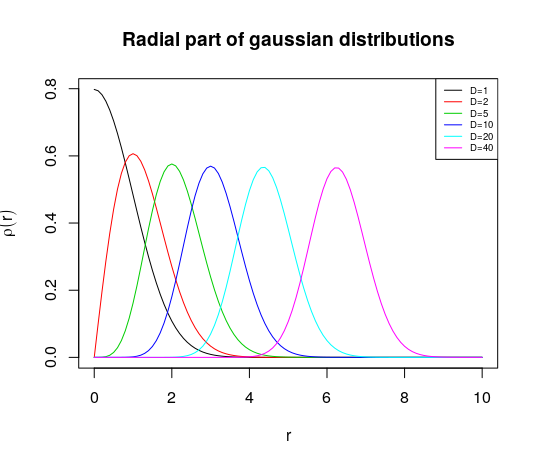
\includegraphics{c1f1}
\end{figure}

It was generated using the following R code.
\begin{lstlisting}[language=R, frame=single]
# Surface area of a unit hypersphere of D dimensions.
surface_area <- function(D) {
  2 * pi^(D/2)/gamma(D/2)
}

rho <- function(D, r) {
  surface_area(D) * r^(D - 1) * exp(-r^2/2)/(2 * pi)^(D/2)
}

r.vals <- seq(from = 0, to = 10, by = 0.1)

plot(
  r.vals,
  rho(1, r.vals),
  type = "l",
  col = 1,
  xlab = expression(r),
  ylab = expression(rho(r)),
  main = "Radial part of gaussian distributions"
)

plot_p <- function(D, n) {
  lines(r.vals, rho(D, r.vals), col = n)
}

sample_set <- data.frame(dim = c(2, 5, 10, 20, 40),
                         col = c(2, 3, 4, 5, 6))
apply(sample_set, 1, function(x)
  plot_p(x[1], x[2]))
legend(
  "topright",
  legend = paste(sep = "", "D=", c(1, sample_set$dim)),
  col = c(1, sample_set$col),
  lty = rep(1, 6),
  cex = 0.6
)

\end{lstlisting}

\item If $a \le b$, $a^2 \le ab$ and hence $a \le \sqrt{ab}$. Consider equation (1.78) of the book.
Its first term is 
\[
T_1 = \int_{\mathcal{R}_1}p(x, C_2)dx \le \int_{\mathcal{R}_1}\sqrt{p(x, C_1)p(x, C_2)}dx.
\]
This is because if the decision boundaries are correctly set, $p(x, C_2) \le p(x, C_1)$ in the region
$\mathcal{R}_1$. Similarly, the second term is
\[
T_2 = \int_{\mathcal{R}_2}p(x, C_1)dx \le \int_{\mathcal{R}_2}\sqrt{p(x, C_1)p(x, C_2)}dx.
\]
The probability of making a mistake is
\[
T_1 + T_2 \le \int_{\mathcal{R}}\left(p(x, C_1)p(x, C_2)\right)^{1/2}dx,
\]
where the region $\mathcal{R}$ is a union of regions $\mathcal{R}_1$ and $\mathcal{R}_2$.

\item The matrix $((L_{ij}))$ has all ones except the main diagonal which has all zeros. A
new $x$ is assigned to class $j$ for which the quantity
\[
\sum_{k}L_{kj}p(C_k|x) = \sum_k (1 - \delta_{kj})p(C_k|x) = \sum_k p(C_k|x) - p(C_j|x) = 1 - p(C_j|x)
\]
is minimal. Therefore, we end up selecting the class for which the posterior probability
is maximal.

\item We cannot classify unless we have the posterior probability $p(C_k|x)$. According to equation
(1.81), we choose that $j$ for which the quantity $\sum_k L_{kj}p(C_k|x)$ is minimal. The 
criterion can be written as
\[
i = \argmin_{1 \le j \le K}\left\{\sum_k L_{kj}p(C_k|x)\right\},
\]
where $K$ is the total number of classes.

\item The problem states that the loss incurred in the reject option is $\lambda$. In other
words, if the expected loss exceed $\lambda$ then we do not classify. Thus, we select class 
$C_i$ if
\[
i = \argmin_{1 \le j \le K}\left\{\sum_k L_{kj}p(C_k|x)\right\},
\]
and if 
\[
\sum_{k} L_{ki}p(C_k|x) < \lambda.
\]
If $L_{ki} = 1 - \delta_{ki}$ then the previous inequality is
\[
1 - \sum_{k}\delta_{ki}p(C_k|x) = 1 - p(C_i|x) < \lambda 
\]
which is equivalent to $p(C_i|x) > 1 - \lambda$. Recall, that this is the criterion for 
selection \emph{without} invoking the reject option. The reject option is invoked when
$p(C_i|x) \le 1 - \lambda$. Thus $\theta$ mentioned in section 1.5.3 is the same as $1 - \lambda$.

\item The expectation value of the loss is
\[
\ev(L(t, y(x))) = \iint \norm{y(x) - t}^2p(x, t)dxdt,
\]
where $x \in \sor^n$, $t \in \sor^m$ and $y:\sor^n \to \sor^m$. We can write $\norm{y(x) - t}^2 =
(y^T(x) - t^T)(y(x) - t)$ so that the functional derivative of this equation with respect to $y(x)$ is
\[
\frac{\delta}{\delta y(x)}\norm{y(x) - t}^2 = 2(y(x) - t).
\]
Then
\[
\frac{\delta\ev(L(t, y(x)))}{\delta x} = 2\int (y(x) - t)p(x,t)dt.
\]
At an extremum,
\[
\int (y(x) - t)p(x, t)dt = 0,
\]
or $y(x) = \int t p(x, t)dt = \ev_t(t|x)$.

\item We write the norm $N = \norm{y(x) - t}^2$ as 
\begin{eqnarray*}
N &=& \norm{y(x) - \ev_t(t|x) + \ev_t(t|x) - t}^2 \\
 &=& \norm{y(x) - \ev_t(t|x)}^2 + \norm{\ev_t(t|x) - t}^2 + \\
 & & (y(x) - \ev_t(t|x))^T(\ev(t|x) - t) + (\ev(t|x) - t)^T(y(x) - \ev_t(t|x)).
\end{eqnarray*}

The third term, after multiplying with $p(x,t)$ and integrated with respect to $t$ is
\[
\int (y(x) - \ev_t(t|x))^T(\ev(t|x) - t)p(x, t)dt = (y(x) - \ev_t(t|x))\left(\ev_t(t|x)\cdot 1 - \int t p(x,t)dt\right) 
\]
The second factor on the right hand side is zero because of which the integral vanishes. Note
that $\ev_t(x|t)$ is a function of $x$.

The fourth term is just the transpose of the third term and therefore vanishes. Therefore,
\[
\ev(L(t, y(x))) = \iint\norm{y(x) - \ev_t(t|x)}^2dxdt + \iint\norm{\ev_t(t|x) - t}^2dxdt.
\]
The only way to minimize the left hand side over the function $y$ is to let it be equal to $\ev_t(t|x)$.
This leaves the irreducible loss as
\[
\ev(L(t, y(x))) = \iint\norm{\ev_t(t|x) - t}^2dxdt.
\]

\item From equation (1.91),
\[
\ev(L_1) = \iint |y(x) - t|p(x, t)dxdt = \int_{\sor^n}\int_{\sor}|y(x) - t|p(x,t)dxdt,
\]
where we have assumed that $x \in \sor^n, t \in \sor$ and $y: \sor^n \to \sor$. We can split
the integral over $t$ to ensure that the integrand is always positive. Thus,
\[
\ev(L_1) = \int_{\sor^n}\int_{-\infty}^{y(x)} (y(x) - t)p(x, t)dxdt + \int_{\sor^n}\int_{y(x)}^{\infty}(t - y(x))p(x, t)dxdt.
\]
We now take the functional derivative with respect to $y(x)$ to get
\[
\frac{\delta\ev(L_1)}{\delta y(x)} = \int_{-\infty}^{y(x)}p(x,t)dt - \int_{y(x)}^{\infty}p(x, t)dt.
\]
At the extremum, the left hand side vanishes so that
\[
\int_{-\infty}^{y(x)}p(x,t)dt = \int_{y(x)}^{\infty}p(x, t)dt.
\]
Thus, $y(x)$ is the conditional median of $t$ given an $x$.

I do not know of even a passably rigorous argument to conclude that $y(x)$ is the conditional 
mode in the case $q \to 0$.

\item There is another way to infer that $h(p) \propto \ln p$. We use a slightly different notation
from the one used in the text. The relation between the densities is $p(x, y) = p_X(x)p_Y(y)$ and
that between information is $h(p) = h(p_X) + h(p_Y)$. Therefore, $a^{h(p)} = a^{h(p_X)}a^{h(p_Y)}$,
for any real constant $a$. Thus, $a^{h(p)} \propto p$ or $h(p) \propto ln p$, where the constant 
$\ln a$ is absorbed into the constant of proportionality.

We can arrive at the same conclusion by taking logarithm of $p(x,y) = p_X(x)p_Y(y)$.

\item The entropy of a discrete random variable is
\[
H(X) = -\sum_{i=1}^Mp(x_i)\log_2 p(x_i) = \sum_{i=1}^M p(x_i)\log_2\left(\frac{1}{p(x_i)}\right)
\]
Jensen's inequality for concave functions is
\[
f\left(\sum_{i=1}^M \lambda_i x_i\right) \ge \sum_{i=1}^M \lambda_i f(x_i).
\]
Choose $\lambda_i = p_i$, $x_i = 1/p_i$ and $f = \log_2$ so that
\[
\log_2\left(\sum_{i=1}^M p(x_i)\frac{1}{p(x_i)}\right) \ge \sum_{i=1}^M p(x_i)\log_2\left(\frac{1}{p(x_i)}\right).
\]
or $\log_2 M \ge H(X)$. 

Note that $\ln M = \ln 2 \log_2 M$ so that $\ln M < \log_2 M$. Therefore, we cannot conclude
that $\ln M \ge H(X)$.

\item The Kullback-Leibler divergence between distributions $p$ and $q$ is
\[
\kl(p || q) = -\int p(x)\ln\left(\frac{q(x)}{p(x)}\right)dx.
\]
If $p(x) = \mathcal{N}(x|\mu,\sigma)$ and $q(x) = \mathcal{N}(x|m, s)$ then
\begin{eqnarray*}
p(x) &=& \frac{1}{\sqrt{2\pi\sigma^2}}\exp\left(-\frac{(x - \mu)^2}{\sigma^2}\right) \\
q(x) &=& \frac{1}{\sqrt{2\pi s^2}}\exp\left(-\frac{(x - m)^2}{s^2}\right)
\end{eqnarray*}
so that
\[
\frac{q(x)}{p(x)} = \frac{\sigma}{s}\exp\left(\frac{(x - \mu)^2}{\sigma^2} - \frac{(x - m)^2}{s^2}\right)
\]
and hence
\[
\ln\left(\frac{q(x)}{p(x)}\right) = \ln\left(\frac{\sigma}{s}\right) + \frac{(x - \mu)^2}{\sigma^2} - \frac{(x - m)^2}{s^2}
\]
$\kl(p||q)$ is thus the sum of three integrals $I_1, I_2, I_3$, where
\begin{eqnarray*}
I_1 &=& -\ln\left(\frac{\sigma}{s}\right)\int_\sor p(x) dx = -\ln\left(\frac{\sigma}{s}\right) \\
I_2 &=& -\int_\sor \frac{(x - \mu)^2}{\sigma^2} p(x)dx \\
I_3 &=& \int_\sor \frac{(x - m)^2}{s^2}p(x)dx
\end{eqnarray*}
Consider $I_2$. Let $u = (x - \mu)/\sigma$ so that 
\[
I_2 = -\sigma\int_\sor \frac{u^2}{\sigma\sqrt{2\pi}}e^{-u^2/2}du = -\frac{1}{\sqrt{2\pi}}\int_{\sor} u^2 e^{-u^2/2}du.
\]
Using equation \eqref{c1pe9}, we get $I_2 = -1$.
Now consider
\[
I_3 = \int_\sor\frac{(x - m)^2}{s^2}p(x)dx = \int_\sor\frac{(x - \mu + \mu - m)^2}{\sigma^2}\frac{\sigma^2}{s^2}p(x)dx,
\]
or
\[
I_3 = \frac{\sigma^2}{s^2}\left(\int_\sor\frac{(x - \mu)^2}{\sigma^2}p(x)dx + \frac{2(\mu - m)}{\sigma^2}\int_\sor (x-\mu)p(x)dx + \frac{(\mu - m)^2}{\sigma^2}\int_\sor p(x)dx\right)
\]
Of these, the first integral is just $-I_2 = 1$. The second integral vanishes because the integrand
is an odd function around $\mu$ and the limits are symmetric around it. The third integral is $1$ 
following the normalization property of $p$. Therefore,
\[
I_3 = \frac{\sigma^2}{s^2}\left(1 + \frac{(\mu - m)^2}{\sigma^2}\right)
\]
and hence
\[
\kl(p || q) = -\ln\left(\frac{\sigma}{s}\right) - 1 + \frac{\sigma^2}{s^2} + \frac{(\mu - m)^2}{s^2}.
\]
It is easily verified that if $\mu = m$ and $\sigma = s$ then $\kl(p || q)$ vanishes.

\item The mutual information between two random variables, $X$ and $Y$ is
\[
I(X, Y) = H(Y) - H(Y|X).
\]
It is a non-negative quantity so that $H(Y) \ge H(Y|X)$. We also have $H(X, Y) = H(X) + H(Y|X)$
so that $H(Y) \ge H(X, Y) - H(X)$ or $H(X, Y) \le H(X) + H(Y)$. If $X$ and $Y$ are statistically
independent then $I(X, Y) = 0$ from which it immediately follows that $H(X, Y) = H(X) + H(Y)$.

\item We will first argue that if $Y = AX$, where $X, Y \in \sor^n$ are random vectors and $A$ is
a non-singular matrix then $p_Y(y) = \abs{\det{A}}^{-1}p_X(x)$. The probability of $X$ taking a value
in a neighbourhood $dx$ around $x$ is $p_X(x)dx$. This is the same as the probability of $AY$ taking
a value in a neighbourhood $d(Ay) = \abs{\det{A}}dy$ around $y$. Therefore, $p_X(x) = \abs{\det{A}}p_Y(y)$ 
or $p_Y(y) = \abs{\det{A}}^{-1}p_X(x)$.

Since $y = Ax$, we also have $dy = \abs{\det{A}}dx$. Therefore,
\begin{eqnarray*}
H(Y) &=& -\int p_Y(y)\ln p_Y(y)dy \\
     &=& -\int \abs{\det{A}}^{-1}p_X(x)\left(\ln\abs{\det{A}}^{-1} + \ln p_X(x)\right)\abs{\det{A}}dx \\
     &=& -\ln\abs{\det{A}}^{-1}\int p_X(x)dx - \int p_X(x)\ln p_X(x)dx \\
     &=& \ln\abs{\det{A}} + H(X).
\end{eqnarray*}

\item The conditional entropy $H(Y|X)$ between two discrete random variables $X$ and $Y$ is
\[
H(Y|X) = \sum_{x, y} p(x, y)\log\left(\frac{p(x, y)}{p(x)}\right).
\]
It is zero if and only if $p(x, y) = p(x)$ or that $p(y|x) = 1$. The latter is true if and only if
$Y$ is a function of $X$.

\item Consider the functional
\[
\begin{split}
f[p] =& -\int_\sor p(x)\ln p(x)dx - \lambda_1\left(\int_\sor p(x)dx - 1\right) \\
      & -\lambda_2\left(\int_\sor xp(x)dx - \mu\right) - \lambda_3\left(\int_\sor (x - \mu)^2p(x)dx - \sigma^2\right)
\end{split}
\]
Note that we have flipped the signs of the multipliers to ensure that the form of $p$ allows 
us to integrate it over $\sor$. The functional derivative of $f$ with respect to $p$ involves 
the following results,
\begin{eqnarray*}
I[p] = \int_\sor f(x)p(x)dx &\Rightarrow& \frac{\delta I}{\delta p} = f(x) \\
J[p] = \int_\sor p(x)\ln p(x)dx &\Rightarrow& \frac{\delta J}{\delta p} = 1 + \ln p(x).
\end{eqnarray*}
We will prove them after solving this problem. Thus,
\[
\frac{\delta f}{\delta p} = -1 - \ln p(x) - \lambda_1 - \lambda_2 x - \lambda_3 (x - \mu)^2.
\]
The functional derivative is zero when $\ln p(x) = -1 - \lambda_1 - \lambda_1 x - \lambda_3(x - \mu)^2$ 
or when
\[
p(x) = \exp\left(-1 - \lambda_1 - \lambda_2 - \lambda_2 (x - \mu)^2\right).
\]

We will now prove the two functional derivative results. Consider 
\[
I[p + \epsilon\eta(x)] = \int_\sor p(x)f(x)dx + \epsilon\int_\sor \eta(x)f(x)dx = I[p] + \epsilon\int_\sor\eta(x)f(x)dx
\]
so that
\[
\frac{\delta I}{\delta p} = f(x).
\]

Now consider
\[
J[p(x) + \epsilon\eta(x)] = \int_\sor p(x)\ln p(x)dx + \epsilon\int_\sor\eta(x)(1 + \ln p(x))dx,
\]
where we have ignored terms of second and higher orders in $\epsilon$. Therefore,
\[
\frac{\delta J}{\delta p} = 1 + \ln p(x).
\]

We now substitute (1.108) into the constraint equation (1.105), (1.106) and (1.107) to get
values of the three unknown Lagrange multipliers. The normalization constraint implies that
\begin{equation}\label{c1pe20}
\int_\sor e^{-\lambda_2 x - \lambda_3(x - \mu)^2}dx = e^{1 + \lambda_1}.
\end{equation}
The integral on the left hand side is evaluated after two changes in variable. Let $u = x - \mu$.
Then the integral, let us call it $I_1$ becomes
\[
I_1 = e^{-\lambda_2\mu}\int_\sor e^{-\lambda_2 u - \lambda_3 u^2}du
\]
We can write the integrand as
\[
\exp\left(-\lambda_3 u^2 - \lambda_2 u\right) = \exp\left[-\left(u\sqrt{\lambda_3} + \frac{\lambda_2}{2\sqrt{\lambda_3}}\right)^2 + \frac{\lambda_2^2}{4\lambda_3}\right]
\]
so that
\[
I_1 = \exp\left(-\lambda_2\mu + \frac{\lambda_2^2}{4\lambda_3}\right)\int_\sor\exp\left[-\left(u\sqrt{\lambda_3} + \frac{\lambda_2}{2\sqrt{\lambda_3}}\right)^2\right]du.
\]
We next introduce the variable
\[
v = u\sqrt{\lambda_3} + \frac{\lambda_2}{2\sqrt{\lambda_3}}
\]
so that
\[
I_1 = \exp\left(-\lambda_2\mu + \frac{\lambda_2^2}{4\lambda_3}\right)\frac{1}{\sqrt{\lambda_3}}\int_\sor e^{-v^2}dv
\]
or
\begin{equation}\label{c1pe21}
I_1 = \exp\left(-\lambda_2\mu + \frac{\lambda_2^2}{4\lambda_3}\right)\sqrt{\frac{\pi}{\lambda_3}}.
\end{equation}
From equations \eqref{c1pe20} and \eqref{c1pe21} we get
\begin{equation}\label{c1pe22}
1 + \lambda_1 + \lambda_2\mu - \frac{\lambda_2^2}{4\lambda_3} = \ln\sqrt{\frac{\pi}{\lambda_3}}.
\end{equation}

The constraint of equation (1.107) gives
\[
\int_\sor (x - \mu)^2e^{-\lambda_2 x - \lambda_3(x - \mu)^2}dx = \sigma^2 e^{1 + \lambda_1}.
\]
Let us denote by $I_3$ the integral on the left hand side. By using the same changes in variables
as before we get
\begin{equation}\label{c1pe23}
\exp\left(-\lambda_2\mu + \frac{\lambda_2^2}{4\lambda_3}\right)\frac{\sqrt{\pi}}{2\lambda_3^{3/2}}\left(1 + \frac{\lambda_2^2}{4\lambda_3}\right) = \sigma^2 e^{1 + \lambda_1}.
\end{equation}
We arbitrarily select $\lambda_2 = 0$ so that equations \eqref{c1pe22} and \eqref{c1pe23} become
\begin{eqnarray*}
1 + \lambda_1 &=& \ln\sqrt{\frac{\pi}{\lambda_3}} \\
\frac{\sqrt{\pi}}{2\lambda_3^{3/2}} &=& \sigma^2 e^{1 + \lambda_1}
\end{eqnarray*}
We can readily solve these equations to get $\lambda_1 = \ln\sqrt{2\pi\sigma^2} - 1$ and 
$\lambda_3 = (2\sigma^2)^{-1}$. The density $p$ is then
\[
p(x) = \frac{1}{\sqrt{2\pi\sigma^2}}\exp\left(-\frac{(x - \mu)^2}{2\sigma^2}\right).
\]

\item If $p$ is a univariate normal distribution,
\[
\ln p = \ln\left(\frac{1}{\sqrt{2\pi\sigma^2}}\right) - \frac{(x - \mu)^2}{2\sigma^2}
\]
and hence
\[
H = -\ln\left(\frac{1}{\sqrt{2\pi\sigma^2}}\right)\int_\sor p(x)dx + \frac{1}{2\sigma^2}\int_\sor (x - \mu)^2 p(x)dx.
\]
Using the constraints of equations (1.105) and (1.107) we get
\[
H = \frac{1}{2}\ln(2\pi\sigma^2) + \frac{1}{2} = \frac{1}{2}[1 + \ln(2\pi\sigma^2)].
\]

\item We first develop a convenient definition of the second derivative.
\begin{eqnarray*}
f^\prime(x) &=& \lim_{k \to 0}\frac{f(x+k) - f(x)}{k} \\
f^\prime(x+h) &=& \lim_{k \to 0}\frac{f(x+h+k) - f(x+h)}{k}
\end{eqnarray*}
Then,
\[
f^{\prime\prime}(x) = \lim_{h \to 0}\frac{f^\prime(x+h) - f^\prime(x)}{h} = \lim_{h,k \to 0}\frac{f(x+h+k) - f(x+h) - f(x+k) + f(x)}{hk}.
\]
Now choose $k = -h$ so that
\begin{equation}\label{c1pe24}
f^{\prime\prime}(x) = \lim_{h \to 0}\frac{f(x+h) + f(x-h) - 2f(x)}{h^2}.
\end{equation}
As 
\[
x = \frac{1}{2}(x + h) + \frac{1}{2}(x - h),
\]
the convexity of $f$ implies that
\[
f(x) \le \frac{1}{2}f(x+h) + \frac{1}{2}f(x-h)
\]
Using this in equation \eqref{c1pe23} proves that $f^{\prime\prime}(x) \ge 0$.

\item We start with
\[
H(X, Y) = \iint p(x, y)\ln p(x, y)dxdy.
\]
Since $p(x, y) = p(y|x)p(x)$,
\begin{eqnarray*}
H(X, Y) &=& \iint p(x, y)\ln p(y|x)dxdy + \iint p(x, y)\ln p(x)dxdy \\
 &=& H(Y|X) + \int\left(\int p(x, y)dy\right)\ln p(x)dx \\
 &=& H(Y|X) + H(X).
\end{eqnarray*}

\item We can write left hand side of (1.115) as
\[
f\left(\lambda_1 x_1 + \sum_{i=2}^{M-1}\lambda_i x_i\right).
\]
But induction hypothesis we can conclude that
\[
f\left(\lambda_1 x_1 + \sum_{i=2}^{M-1}\lambda_i x_i\right) \le f(\lambda_1 x_1) + f\left(\sum_{i=2}^{M} \lambda_i x_i\right).
\]
We can use the induction hypothesis once again on the second term to get the desired result.

\item 
\begin{enumerate}
\item $H(X) = -\frac{2}{3}\ln\frac{2}{3} - \frac{1}{3}\ln\frac{1}{3}$.
\item $H(Y) = -\frac{1}{3}\ln\frac{1}{3} - \frac{2}{3}\ln\frac{2}{3}$.
\item $H(Y|X) = -\sum_{x,y} p(x, y)\ln p(y|x) = -\frac{1}{3}\ln\frac{1}{2} - \frac{1}{3}\ln\frac{1}{2} - 0 - \frac{1}{3}\ln 1$.
\item $H(X|Y) = -\sum_{x,y} p(x, y)\ln p(x|y) = -\frac{1}{3}\ln 1 - 0 - \frac{1}{3}\ln\frac{1}{2} - \frac{1}{3}\ln\frac{1}{2}$.
\item $H(X, Y) = -\ln\frac{1}{3}$.
\item The definition of mutual information is
\[
I(X, Y) = -\sum_{x,y}p(x, y)\ln\frac{p(x)p(y)}{p(x, y)}.
\]
Therefore,
\[
I(X, Y) = -\frac{1}{3}\ln\frac{\frac{2}{3}\frac{1}{3}}{\frac{1}{3}} - \frac{1}{3}\ln\frac{\frac{2}{3}\frac{2}{3}}{\frac{1}{3}} - \frac{1}{3}\ln\frac{\frac{1}{3}\frac{2}{3}}{\frac{1}{3}}.
\]
\end{enumerate}

\item Since $\log$ is a concave function,
\[
\log\left(\frac{x_1}{2} + \frac{x_2}{2}\right) \ge \frac{1}{2}\log x_1 + \frac{1}{2}\log x_2 = \log\sqrt{x_1x_2}.
\]

\item Since $p(x, y) = p(y|x)p(x)$,
\begin{eqnarray*}
I(X, Y) &=& -\iint p(x, y)\ln\left(\frac{p(y)}{p(y|x)}\right)dxdy \\
 &=& -\iint p(x, y)\ln p(y) dxdy - \iint p(x, y)\ln p(y|x)dxdy.
\end{eqnarray*}
The first term on extreme right can be written as
\[
-\int\left(\int p(x, y)dx\right)\ln p(y)dy = -\int p(y)\ln p(y)dy = H(Y).
\]

\end{enumerate}

